\documentclass[oneside,final,14pt,a4paper]{extreport}

\usepackage{tempora} % Times New Roman alike font  

\usepackage{vmargin}
\setpapersize{A4}
\setmarginsrb{2.5cm}{2.2cm}{2.2cm}{2.2cm}{0pt}{10mm}{0pt}{13mm}
\usepackage{setspace}
\setstretch{1.5}
\usepackage{indentfirst}
\parindent=1.25cm

%%%%% ADDED TO SUPPORT TT BOLD FACES %%%%
\DeclareFontShape{OT1}{cmtt}{bx}{n}{<5><6><7><8><9><10><10.95><12><14.4><17.28><20.74><24.88>cmttb10}{}
\renewcommand{\ttdefault}{pcr}
%%%%% END %%%%%%%%%%%%%%%%%%%%%%%%%%%%%%% 

\usepackage{atbegshi,picture}
% \usepackage[T1,T2A]{fontenc}
\usepackage{fontspec}
\setmainfont{Times New Roman}

\usepackage[utf8]{inputenc}

\usepackage[english]{babel}
\usepackage[backend=biber,style=ieee,autocite=inline]{biblatex}
\bibliography{ref.bib}
\DefineBibliographyStrings{english}{%
  bibliography = {References},}
\usepackage{blindtext}

\usepackage[nottoc]{tocbibind}

\usepackage{microtype}    
\usepackage{pdfpages}
\newenvironment{bottompar}{\par\vspace*{\fill}}{\clearpage}
\usepackage{amsmath}
\usepackage{amsfonts}
\usepackage{amssymb}
\usepackage{mathtools}
\usepackage{url}
\usepackage[most]{tcolorbox}
\usepackage{ascii}
\usepackage{relsize}
\usepackage{tikz}  
\usepackage{xspace}
\usetikzlibrary{positioning, arrows.meta}

\usepackage{amsthm}
\newtheorem{theorem}{Theorem}
\newtheorem{corollary}{Corollary}
\newtheorem{lemma}{Lemma}
\newtheorem{proposition}{Proposition}
\theoremstyle{definition}
\newtheorem{definition}{Definition}
\theoremstyle{remark}
\newtheorem*{remark}{Remark}
\theoremstyle{remark}
\newtheorem*{example}{Example}

% \usepackage{titlesec}
\usepackage{float}
\usepackage{graphicx}
\graphicspath{{figs/}} %path to images
\usepackage{array}
\usepackage{multirow,array}
\usepackage{caption}
\usepackage{subcaption}
\usepackage{hyperref}
\hypersetup{
	colorlinks=true,
	linkcolor=black,
	citecolor=black,
	urlcolor=black
}
\usepackage{paralist}
\usepackage{listings}
\usepackage{zed-csp}
\usepackage{fancyhdr}
\usepackage{csquotes}
\usepackage{color}
% \usepackage{anyfontsize}
% \usepackage{mathptmx}
% \usepackage{t1enc}
\usepackage{syntax}
\usepackage{chngcntr}
\usepackage{upgreek}
\usepackage{bm}
\usepackage{multicol}
% \usepackage{hyperref}
\usepackage{booktabs}
\usepackage{multirow}
\usepackage{longtable}
\usepackage[font=singlespacing, labelfont=bf]{caption}
% \counterwithout{table}{chapter}
% \renewcommand{\thetable}{\Roman{table}}
%Hints
\newcommand\pic[1]{(Fig. \ref{#1})} %Ref on figure
\newcommand\tab[1]{(Tab. \ref{#1})} %Ref on table

\setlength{\headheight}{32.0976pt}
\usepackage{enumitem}
\newlist{inlinelist}{enumerate*}{1}
\setlist*[inlinelist,1]{%
  label=(\arabic*),
}

% \setcounter{secnumdepth}{4}
\captionsetup[table]{labelfont={normalfont}, name={TABLE}, labelsep={newline}}
\setlength{\parindent}{2em} 
\DeclareCaptionLabelSeparator{figSep}{.\quad}
\captionsetup[figure]{
  labelfont={bf}, 
  name={Fig.}, 
  labelsep=period, 
  justification=raggedright, 
  singlelinecheck=false, 
}
\counterwithin{figure}{chapter}

% \usepackage{titlesec}
% \titleformat{\section}[hang]{\fontsize{20}{24}\selectfont\filcenter}{\Roman{section}}{1em}{}
% \titleformat{\subsection}[hang]{\itshape}{\Alph{subsection}.}{1em}{}[]
% \titleformat{\subsubsection}[runin]{\itshape}{\arabic{subsubsection})}{1em}{}[$:$]
% \titlespacing{\subsubsection}{1em}{1em}{1em}
% \titleformat{\paragraph}[runin]{\itshape}{\alph{paragraph})}{1em}{}[$:$\quad]
% \titlespacing{\paragraph}{2em}{1em}{1em}

\usepackage{placeins} % for \FloatBarrier

\pagestyle{fancyplain}

% remember section title
\renewcommand{\chaptermark}[1]%
{\markright{\thechapter\ #1}{}}

% subsection number and title
\renewcommand{\sectionmark}[1]%
	{\markright{\thesection\ #1}}

\rhead[\fancyplain{}{\bf\leftmark}]%
      {\fancyplain{}{\bf\thepage}}
\lhead[\fancyplain{}{\bf\thepage}]%
      {\fancyplain{}{\bf\rightmark}}
\cfoot{} %bfseries


\newcommand{\dedication}[1]
   {\thispagestyle{empty}
     
   \begin{flushleft}\raggedleft #1\end{flushleft}
}



\usepackage{cleveref}
\crefname{table}{table}{tables}
\Crefname{table}{Table}{Tables}
\crefname{figure}{Fig.}{figures}
\Crefname{figure}{Fig.}{Figures}
\crefname{listing}{List.}{List.}
\Crefname{listing}{List.}{List.}
\crefname{section}{Sec.}{Sec.}
\Crefname{section}{Sec.}{Sec.}
\Crefname{equation}{Eq.}{Eq.}
\crefname{equation}{Eq.}{Eq.}
\crefname{chapter}{Ch.}{Ch.}


\usepackage{epigraph}

% --- START --- minted

% https://github.com/latextemplates/IEEE/blob/main/paper-conference-minted.tex
\usepackage[newfloat]{minted}
\setminted{
  % Add line numbers, can be added per listing 
  % linenos=true,
  % Line numbers not flowing out of the margin
  numbersep=12pt,
  xleftmargin=19pt,
  breaklines=true,
  breakbytoken=true,
  % For the very long tokens, use
  % "breakanywhere, breakbytokenanywhere=false"
  % on the listing level. Otherwise breakanywhere will not have any effect.
  breakbytokenanywhere=true
}
\renewcommand{\theFancyVerbLine}{\textcolor{gray}{\arabic{FancyVerbLine}}}

\captionsetup[listing]{labelfont={normalfont}, name={List.}, labelsep=period}
\counterwithout{listing}{chapter}

\newcommand{\hs}{\mintinline[fontsize=\normalsize]{haskell}}

% --- END --- minted

% \setcounter{secnumdepth}{4}
% \captionsetup[table]{labelfont={normalfont}, name={TABLE}, labelsep={newline}}
% \counterwithout{table}{chapter}
% \renewcommand{\thetable}{\Roman{table}}
% \setlength{\parindent}{2em}
% \DeclareCaptionLabelSeparator{figSep}{.\quad}
% \captionsetup[figure]{labelfont={normalfont}, name={Fig.}, labelsep=period}
% \counterwithout{figure}{chapter}


% don't break citations
\let\oldcite\cite
\renewcommand{\cite}[2][]{\mbox{\oldcite[#1]{#2}}}

\newcommand{\fig}[4]{
  \begin{figure}[h]
    \centering
    \includegraphics[scale=0.35]{#1}
    \caption{#2}
    \label{fig:#3}
  \end{figure}
}

\newcommand{\Arralac}{\texttt{Arralac}\xspace}

\begin{document}

\includepdf[noautoscale,offset=75 -75,pages=-]{title.pdf}

% \setcounter{page}{2}

\tableofcontents

\cleardoublepage
\listoftables

\cleardoublepage
\listoffigures

\cleardoublepage
\begin{abstract}

    Advanced type systems, such as arbitrary-rank polymorphism, are powerful but notoriously difficult to implement, creating a pedagogical gap between seminal theory, like that of Peyton Jones et al., and complex production compilers like the Glasgow Haskell Compiler (GHC). This thesis addresses this gap by presenting \Arralac, a small, tutorial-focused compiler for a lambda calculus with arbitrary-rank polymorphism. Rather than replicating the eager unification algorithm of foundational papers, \Arralac implements a modern, GHC-style, two-phase architecture that cleanly separates constraint generation from constraint solving, demonstrating a more modular and pedagogically clear approach. This design is supported by a Trees That Grow (TTG) Abstract Syntax Tree (AST), which enables pass-specific annotations crucial for tooling. The system is delivered as a complete, interactive toolchain, featuring a Language Server Protocol (LSP) implementation that makes the internal state of the typechecker transparent and explorable within a code editor. The implementation is validated by its ability to correctly handle higher-rank types, reject invalid programs through level-based skolem escape checks, and ultimately demonstrates that a constraint-based model serves as a clearer instructional tool than its eager counterpart. By synthesizing foundational theory with modern engineering patterns and interactive feedback, \Arralac provides an accessible and effective resource that demystifies a cornerstone of advanced compiler design.

\end{abstract}

% Depend on above part

\setcounter{page}{8}

% set manually the number, from which Chapter 1 starts!
% Why do we put 7 in this case?
% Title page - page 1
% Contents - page 2, page 3
% List of tables - page 4
% List of figures - page 5
% Abstract - page 6
% Chapter 1 - page 7
% In your thesis the counter number can be different, please count carefully and insert the corresponding number.

\chapter{Introduction}
\label{chap:Introduction}

\epigraph{Any sufficiently advanced technology is indistinguishable from magic.}{\textit{Arthur C. Clarke}}

For us, that ``sufficiently advanced technology'' was the Glasgow Haskell Compiler (GHC) \cite{ghc-site}.
Although we had been programming in Haskell for several years before we started working on the thesis, we somehow were not curious enough to learn about the internals of the Haskell compiler.

% TODO add links to the resources?
Luckily, the compiler had open source code, its implementation was based on scientific publications, the project wiki and online presentations about the compiler were insightful, and there were online communities where the compiler developers and other knowledgeable people were ready to answer our questions.

To improve our understanding of the compiler internals and make an excuse for  writing some more Haskell, we decided to implement a small extensible typed functional language using approaches similar to those employed in GHC.

These approaches included using a fancy abstract syntax tree (AST) representation, support for higher-rank types, a bidirectional type inference algorithm, collecting and then solving type constraints, translation to a core language based on System F, and interpretation of that language.

Additionally, we decided to study available options for the AST representation and the the type inference engine to educate ourselves and possibly use in our project. For example, we learned about the Free Foil approach \cite{kudasov-free-2024} that enabled type-safe capture-avoiding substitution and could be used to represent types or the core language.

% TODO convert to references
As we wanted to iterate on the language syntax quickly, we decided to use the BNFC parser generator \cite{bnfc-parser-generator} instead of the combination of Happy and Alex used in the GHC \cite{ghc-2025}.

At the end, we expected to obtain a parser, a type inference engine, an interpreter, a language server, and a VS Code extension for our language.

We could not find on GitHub any well-documented implementation of a very simple language featuring predicative higher-rank polymorphism, having the mentioned components, and resembling the GHC. In our work, we attempted to partially close this gap by documenting the considered options and explaining our final implementation. The implementation \cite{deemp-higher-rank-free-foil} is available on GitHub under the MIT license.

\newpage

\section{Overview}

The \cref{chap:LiteratureReview} reviews several AST representations and type inference algorithms including the ones that we chose for our implementation.
Then, \cref{chap:DesignImplementation} explains the theoretical basis and details of the implementation of our language.
Next, \cref{chap:EvaluationDiscussion} summarizes the obtained results and describes the development experience.
Following that, \cref{chap:Conclusion} mentions possible directions for future work.
Finally, \cref{chap:Appendix} provides a number of snippets mentioned in our work.


\chapter{Literature Review}
\label{chap:LiteratureReview}

We studied several abstract syntax tree representations (\cref{sec:AstRepresentations}) and type inference algorithms (\cref{sec:TypeInferenceAlgorithm}) to understand which ones could be used in different parts of our implementation.

\section{Technical constraints}
\label{chap:LiteratureReview:sec:AstRepresentations:TechnicalConstraints}

\begin{itemize}
    \item We thought about extending our language to support modules, integer and floating-point numbers, and record types in future.
    \item We wanted to be able to freely use mutually recursive data types for different categories of AST nodes. For example, such categories could be modules and statements. A module could contain a number of statements and a statement could introduce a module.
    \item For the language server, we needed to annotate some of the AST nodes with additional information such as locations of the source code that corresponded to these nodes and types of expressions represented by these node subtrees.
    \item We used the BNFC parser generator that generated an AST data type parameterised by an annotation type variable.
          % TODO not only start position - see https://github.com/BNFC/bnfc/pull/463
          After parsing, the annotation of almost each AST node contained the position of a source code span parsed to produce that node.
\end{itemize}

\section{AST representations}
\label{sec:AstRepresentations}

For the AST representation, we could use the data types produced by the parser generator BNFC (\cref{chap:LiteratureReview:sec:AstRepresentations:BnfcAst}), \texttt{hypertypes} (\cref{chap:LiteratureReview:sec:AstRepresentations:Hypertypes}) and alternative representations described in that project, \texttt{compdata} (\cref{chap:LiteratureReview:sec:AstRepresentations:Compdata}), the Free Foil (\cref{chap:LiteratureReview:sec:AstRepresentations:FreeFoil}), or the Trees that grow approach (\cref{chap:LiteratureReview:sec:AstRepresentations:TreesThatGrow}).

\subsection{BNFC AST}
\label{chap:LiteratureReview:sec:AstRepresentations:BnfcAst}

The BNFC-generated parsers did not support parsing signed integer numbers out of the box.
Our workaround was to define a \texttt{token}, then use that \texttt{token} to parse code and construct a node containing a string in the correct format, then post-process the parsed AST to replace nodes containing such raw values with \texttt{internal} (not parsable) nodes containing numbers.

\begin{minted}{haskell}
token IntegerSigned  ('-'? digit+) ;
LitIntegerRaw.       Object ::= IntegerSigned ;
internal LitInteger. Object ::= IntegerSigned ;
\end{minted}

It was inconvenient though that both variants of nodes were in the AST and we would have to pattern-match on the \texttt{LitIntegerRaw} even if that variant of node was completely unnecessary after the post-processing.

\subsection{\texttt{hypertypes}}
\label{chap:LiteratureReview:sec:AstRepresentations:Hypertypes}

The \texttt{hypertypes} package \cite{hypertypes-hackage} let users construct expressions from individual components like in the Data types à la carte \cite{swierstra-data-2008} approach. These components could be mutually recursive types like in \texttt{multirec} \cite{multirec-hackage} and could be processed via type classes. The package description explained the limitations of several previous approaches.

The package provided primitives for annotating nodes (\href{https://hackage.haskell.org/package/hypertypes-0.2.2/docs/Hyper-Combinator-Ann.html}{\texttt{Hyper.Ann}}), for constructing typed lambda calculus expressions (\href{https://hackage.haskell.org/package/hypertypes-0.2.2/docs/Hyper-Syntax.html}{\texttt{Hyper.Syntax}}), and for unification (\href{https://hackage.haskell.org/package/hypertypes-0.2.2/docs/Hyper-Unify.html}{Hyper.Unify}). The \href{https://github.com/lamdu/hypertypes/blob/06cf48ef9c85c54cbe722a448754cb89931b23e7/src/Hyper/Diff.hs}{\texttt{Hyper.Diff}} module showed how to annotate trees and the \href{https://github.com/lamdu/hypertypes/tree/06cf48ef9c85c54cbe722a448754cb89931b23e7/test/TypeLang.hs}{\texttt{TypeLang}} module provided an implementation of type inference for a language with row-types using the primitives provided by the package.

\subsection{\texttt{compdata}}
\label{chap:LiteratureReview:sec:AstRepresentations:Compdata}

Likewise, the \texttt{compdata} package \cite{compdata-hackage} supported mutually recursive data types, including GADTS (\texttt{Data.Comp.Multi}).
Provided examples showed (\href{https://github.com/pa-ba/compdata/blob/e916a9ae847b37d7932669f9365de987d09fd9e0/src/Data/Comp/Multi.hs#L322
}{example1}, \href{https://github.com/pa-ba/compdata/blob/e916a9ae847b37d7932669f9365de987d09fd9e0/examples/Examples/Multi/Desugar.hs}{example2}, \href{https://gist.github.com/liarokapisv/bb857a23ecd9df945690f73e0acfbe80}{example3} related to this \href{https://github.com/pa-ba/compdata/issues/35}{issue}) how to use annotated ASTs.

\section{Stitch}

\citeauthor{eisenberg-stitch-2020} explored an implementation of a simply typed $\lambda$-calculus with a non-typechecked AST with type-level de Bruijn indices that enforced the construction of only well-scoped terms during parsing and a type-checked AST indexed with type-level contexts and node types. The implementation uses lots of Haskell extensions and can be a good playground for studying them in action.

\section{Free Foil}
\label{chap:LiteratureReview:sec:AstRepresentations:FreeFoil}

The Free Foil \cite{kudasov-free-2024} approach by \citeauthor{kudasov-free-2024} implemented in the \cite{free-foil-hackage} package allowed for constructing an AST where nodes were indexed with a phantom type variable denoting the scope. Each node represented either a variable or any other language construct, potentially scoped under a (single) binder that extended the scope. The approach enabled type-safe capture-avoiding substitution of variables for expressions. Additionally, it allowed to define generic recursive AST processing functions that could be used for any AST where nodes were constructed from a user-supplied type (\texttt{sig}) that had necessary type class instances such as \texttt{Bifunctor}.

The example in \href{https://hackage.haskell.org/package/free-foil-0.2.0/docs/Control-Monad-Free-Foil-Example.html}{Control.Monad.Free.Foil.Example} showed a definition of an AST for an untyped lambda calculus. The pattern synonym \href{https://hackage.haskell.org/package/free-foil-0.2.0/docs/src/Control.Monad.Free.Foil.Example.html#LamE}{\texttt{LamE}} was used to construct expressions under a binder.

The Free Foil approach had two limitations that could be inconvenient given our Technical constraints (\cref{chap:LiteratureReview:sec:AstRepresentations:TechnicalConstraints}).

First, the last library version required that mutually recursive types in the AST be combined into a single data type. The library author stated that the library could theoretically support mutually recursive types if another representation were used.

% TODO link to the definition of lexical scoping
Second, it could increase the AST size if our language had modules, or, more generally, supported non-lexical scoping.
In a language with modules, relating the variable declaration and usage sites may require performing multi-phased type checking, e.g., using the scope graphs approach \cite{poulsen-monadic-2023}.
If we wanted to use binders to track the declaration sites, after parsing, we would need to construct an AST with nodes for modules and without binders, then type check that AST, and then construct an AST with resolved binders.
In the subtree of each node that denoted a module import, we would need to create nodes that would introduce binders for visible variables from that module.
At the same time, we would still need to track for each binder the module that the variable came from.

\subsection{Trees That Grow}
\label{chap:LiteratureReview:sec:AstRepresentations:TreesThatGrow}

The GHC used a variant of the Trees That Grow \cite{najd-trees-2016} approach (\href{https://gitlab.haskell.org/ghc/ghc/-/wikis/implementing-trees-that-grow/hs-syn}{HsSyn}, \href{https://gitlab.haskell.org/ghc/ghc/-/wikis/implementing-trees-that-grow/trees-that-grow-guidance}{Trees that grow guidance}).

This approach suggests to parameterise a data type with a type variable and use open type families applied to that type variable instead of concrete types for constructor fields. This way, it is possible to specify a different set type family instances and corresponding field types for each instantiation of the parameter. For example, in GHC, the AST is parameterised by the compilation phase (parsed, renamed, typechecked), and the type families are used to disable certain constructors and choose which nodes should have annotations of particular types.

The data type should also have an additional constructor with a field specified in the similar manner using a type family. Then, it will be possible to "add constructors" to the data type by resolving the type of that field to another data type and providing pattern synonyms that would make constructors of another type wrapped in the constructor of the additional field look as if they belong to the initial data type. A similar approach could be used with constructors of the initial data type to "add" fields to these constructors if they provided an additional field represented as an application of a type family.

Unlike Free Foil, this approach supported mutually recursive types and was similar to using an ordinary data type parameterised by a type variable except one had to define quite a lot of type family instances for constructor fields.

\section{Type inference algorithm}
\label{sec:TypeInferenceAlgorithm}

\subsection{GHC}

% TODO more precise number
The current GHC type inference engine has tens of thousands lines of code.
It has been incrementally developed over years to add new extensions to the Haskell type system.
Some of these extensions had accompanying scientific publications.
% TODO proof that it's based on the paper
One of such extensions was \href{https://gitlab.haskell.org/haskell/prime/-/wikis/RankNTypes}{\texttt{RankNTypes}} that enabled arbitrary-rank predicative polymorphism.
The extension was based on \cite{jones-practical-2007} that described a bidirectional type inference algorithm for a type system with arbitrary-rank types. The Technical Appendix \cite{practical-type-inference-proofs} provided the proofs of theorems mentioned in the paper, including the proofs of completeness and soundness, but not of the attached Haskell implementation.

\subsection{New algorithms}

\cite{jones-practical-2007} was published around 20 years ago, and since then, multiple new type inference algorithms outside of the work on the GHC had been published.
Moreover, some of them were implemented in Haskell \cite{github-goldenberg-artem-goldenbergbidirectionalsystem-2025} \cite{github-choi-kwanghoonbidi-2025} \cite{github-chen-cu1ch3ntype-inference-zoo-2025}.

The following sections
% TODO add links to implementations.

\subsection{Bidirectional typing}

There are two modes in bidirectional typing - the inference mode that helps reduce the number of type annotations required from the programmer and propagates the available type information, and the checking mode that can type expressions for which a type could not be inferred otherwise \cite{dunfield-bidirectional-2020}.

In \cite{dunfield-complete-2013}, \citeauthor{dunfield-complete-2013} provided an arguably simple bidirectional type inference algorithm for a system with higher-rank predicative polymorphism. Their algorithm had similar properties \cite[Fig. 15]{dunfield-complete-2013} as the one presented in \cite[Sec.~6]{jones-practical-2007}, namely, it abided the $\eta$-law \cite[Ch.~4]{selinger-lecture-2013} and was sound and complete wrt. the System F \cite[Ch.~8]{selinger-lecture-2013}. The authors argued that using ordered contexts, existential variables, and precise scoping rules in their work were a better fit from the type-theoretic point of view than using the ``bag of constraints" approach, unification variables, and skolemization that were described, e.g., in \cite{jones-practical-2007}.

In a later work \cite{dunfield-sound-2019}, \citeauthor{dunfield-sound-2019} built on \cite{dunfield-complete-2013} and described the type inference algorithm for a significantly extended language that featured existential quantification, sums, products, pattern matching, etc. For their algorithm and proofs, they used a desugared version \cite[Fig. 11]{dunfield-sound-2019} of the surface language \cite[Fig. 1]{dunfield-sound-2019}.

Additionally, \citeauthor{dunfield-bidirectional-2020} extensively surveyed \cite{dunfield-bidirectional-2020} the works on bidirectional typing and supplied a guide to creating new programmer-friendly bidirectional type inference algorithms.

\subsection{Modifications of bidirectional typing}

\citeauthor{xie-higher-rank} \cite{xie-higher-rank} reviews \cite{dunfield-complete-2013} (Sec. 2.3), suggests using the application mode in addition to inference and checking modes (Sec. 3), provides a novel algorithm for kind inference (Sec. 7), and relates it to the current GHC implementation (Sec. 8.6), noting possible points for improvement (Appendix Sec. C).

\citeauthor{xue-contextual-2024} \cite{xue-contextual-2024} explain the limitations of bidirectional typing (Sec 2.5) and generalize bidirectional typing to contextual typing by propagating any necessary contextual information instead of just type information and replacing the two modes (inference and checking) with counters that track the amount of the contextual information to be propagated. Their approach allows to specify exact places in the code where a programmer must provide annotations.

\subsection{Beyond bidirectional typing}

\citeauthor{parreaux-when-2024} suggest a novel non-bidirectional type inference algorithm SuperF that supports first-class (i.e., impredicative) higher-rank polymorphism. Impredicative polymorphism allows instantiation of type variables with polytypes while predicative allows only monotypes \cite[Sec 3.4]{jones-practical-2007}. The algorithm infers a type for each subterm and then checks against user annotations written in System F syntax. The authors claim that subtype inference used in their approach suits much better for implementing first-class polymorphism than first-order unification-based approaches. As a demonstration of the capabilities of the algorithm, the authors show that it types almost any term even without type annotations (Sec 5.4, Sec 5.5).


\chapter{Design and Methodology}
\label{chap:DesignAndMethodology}

This chapter details the architectural design and core methodologies employed in the implementation of \texttt{Arralac}, a tutorial compiler for a lambda calculus with arbitrary-rank polymorphism. The design is heavily inspired by the bidirectional type inference system described in \textit{Practical type inference for arbitrary-rank types} \cite{jones-practical-2007}, but it incorporates several modern implementation techniques and diverges in key areas to prioritize clarity and extensibility. We will first outline the overall system architecture, then delve into the specifics of the Abstract Syntax Tree (AST) representation and the constraint-based type inference engine.

\section{System Architecture: The Compilation Pipeline}
\label{sec:Design:Pipeline}

The process of transforming a source file from plain text into an evaluated term is managed by a multi-stage pipeline. Each stage performs a distinct transformation on the program representation, passing its output to the next stage. This modular design isolates concerns, simplifies debugging, and facilitates future extensions. Its stages are described below.

\begin{figure}[h!]
    \centering
    \begin{tikzpicture}[
            node distance=1.5cm and 2.5cm,
            auto,
            block/.style={rectangle, draw, fill=blue!20, text width=7em, text centered, rounded corners, minimum height=3em},
            arrow/.style={-Latex, thick}
        ]
        % Define the pipeline stages as nodes
        \node[block] (reader) {Reading};
        \node[block, right=of reader] (parser) {Parsing};
        \node[block, right=of parser] (renamer) {Renaming};
        \node[block, below=of renamer] (typechecker) {Typechecking};
        \node[block, left=of typechecker] (solver) {Solving};
        \node[block, left=of solver] (zonker) {Zonking};
        \node[block, below=of zonker] (core) {Core Conversion};
        \node[block, right=of core] (evaluation) {Evaluation};

        % Draw the arrows connecting the stages
        \draw[arrow] (reader) -- (parser);
        \draw[arrow] (parser) -- (renamer);
        \draw[arrow] (renamer) -- (typechecker);
        \draw[arrow] (typechecker) -- (solver);
        \draw[arrow] (solver) -- (zonker);
        \draw[arrow] (zonker) -- (core);
        \draw[arrow] (core) -- (evaluation);
    \end{tikzpicture}
    \caption{The \texttt{Arralac} Pipeline}
    \label{fig:pipeline}
\end{figure}


\begin{itemize}
    \item \textbf{Reading:} The initial stage reads the source file from disk into a text buffer.
    \item \textbf{Parsing:} The text is passed to a parser generated by BNFC \cite{bnfc-site-2025}, which transforms the linear stream of characters into an initial Abstract Syntax Tree (AST). Each node in this tree is annotated with its location (span) in the source code.
    \item \textbf{Renaming:} This crucial stage performs $\alpha$-conversion by traversing the AST and assigning a unique identifier to every variable binding. This ensures that all occurrences of a variable are unambiguously linked to their binder, resolving issues of shadowing and preparing the program for typechecking.
    \item \textbf{Typechecking:} The renamed AST is traversed to generate a set of type constraints. This pass does not solve the constraints but gathers them, including equality constraints between types and implication constraints that capture the scoping requirements of polymorphism.
    \item \textbf{Solving:} A separate solver pass attempts to unify the generated constraints. It is here that skolem escape and occurs checks are performed. Unsolved metavariables are left as-is.
    \item \textbf{Zonking:} After solving, the AST is "zonked." This pass substitutes all solved metavariables with their inferred types, producing a fully-typed AST. Unsolved metavariables are explicitly marked as such.
    \item \textbf{Core Conversion \& Evaluation:} The final, zonked AST is converted into a simpler Core language representation for evaluation. The evaluator then reduces the Core term to its weak head normal form (WHNF).
\end{itemize}

\section{Abstract Syntax Tree Design}
\label{sec:Design:AST}

The choice of AST representation is a foundational design decision that profoundly impacts the compiler's extensibility and maintainability. My design choices were guided by several key technical constraints:
\begin{itemize}
    \item \textbf{Extensibility:} The AST needed to gracefully accommodate future language extensions, such as new literal types or statement forms, without requiring invasive changes to existing data type definitions.
    \item \textbf{Annotation for Tooling:} To support language server features, it was essential to annotate AST nodes with auxiliary information, particularly the source code span and, after typechecking, the inferred type of the node.
    \item \textbf{Parser Generator Integration:} The design had to integrate smoothly with the ASTs produced by the BNFC parser generator \cite{bnfc-site-2025}.
\end{itemize}

After evaluating several alternatives, including the default BNFC representation, \texttt{hypertypes} \cite{hypertypes-hackage}, and \texttt{compdata} \cite{compdata-hackage}, I selected the \textbf{Trees That Grow (TTG)} pattern \cite{trees-that-grow-2016}. TTG, also used within GHC \cite{ghc-gitlab-2025}, provides an elegant solution to the problem of extensibility by parameterizing data types by the compiler pass and using open type families for fields.

My implementation of TTG differs slightly from GHC's for improved flexibility. Whereas GHC uses concrete types in some fields, my implementation uses type family applications for \textit{all} fields, ensuring that every part of an AST node can be customized for a given compiler pass. This is illustrated in the comparison below.

\begin{minted}[frame=lines,label={GHC's TTG AST Structure (Simplified)}]{haskell}
-- In GHC (compiler/Language/Haskell/Syntax/Expr.hs)
data HsExpr p
  = HsVar (XVar p) (LIdP p) -- LIdP is a type synonym, not a type family
  ...

type LIdP p = XRec p (IdP p)
\end{minted}

\begin{minted}[frame=lines,label={Arralac's TTG AST Structure}]{haskell}
-- In Arralac (Language/Arralac/Syntax/TTG/SynTerm.hs)
data SynTerm x
  = SynTerm'Var (XSynTerm'Var' x) (XSynTerm'Var x) -- All fields use type families
  ...

-- Type families for each field, defined separately
type family XSynTerm'Var' x
type family XSynTerm'Var x
\end{minted}

This uniform use of type families allows, for instance, the type of a variable itself to change between passes—from a simple \texttt{Name} in the `Renamed` pass to a \texttt{TcTermVar} containing a full type in the `Typechecked` pass.

\section{Type Inference and Constraint Solving}
\label{sec:Design:TypeInference}

The core of the compiler is its type inference engine. This section first reviews the foundational concepts from \cite{jones-practical-2007} that underpin the system, and then describes how \texttt{Arralac}'s implementation diverges to adopt a constraint-based approach.

\subsection{Foundations from \textit{Practical Type Inference}}
\label{sec:Design:Foundations}

The algorithm in \cite{jones-practical-2007} provides a practical way to handle higher-rank types by leveraging programmer annotations. Its key mechanisms are as follows:

\begin{itemize}
    \item \textbf{Type Hierarchy:} Types are stratified to manage polymorphism. \textbf{\texttt{tau} ($\tau$)} types are monotypes (no \texttt{forall}). \textbf{\texttt{rho} ($\rho$)} types can have nested polytypes but no top-level \texttt{forall}. \textbf{\texttt{sigma} ($\sigma$)} types are polytypes with a top-level \texttt{forall}. All interaction happens within a \textbf{type context} ($\Gamma$), which maps variables to their $\sigma$-types.

    \item \textbf{Metavariables and Unification:} Inference works by creating placeholder \textbf{metavariables} for unknown types and generating equality constraints. The process of solving these constraints is \textbf{unification}. Crucially, the paper's system operates under a \textbf{monotype invariant}: metavariables can only be unified with $\tau$-types. This predicative restriction is vital for ensuring that type inference is decidable and its result is \textbf{order-independent}.

    \item \textbf{Bidirectional Type Checking:} The algorithm operates in two modes. In \textbf{inference mode} ($\uparrow$), it synthesizes the most general type for an expression. In \textbf{checking mode} ($\downarrow$), it verifies that an expression conforms to a known, expected type. This duality is key: inference is used for simple expressions, but when a higher-rank type is expected (e.g., as a function argument), the system switches to checking mode, pushing the polymorphic type "down" into the expression and avoiding the need for undecidable full inference.

    \item \textbf{Subsumption and Skolemization:} To check if a function of type $\sigma_1$ can be used where $\sigma_2$ is expected (i.e., $\sigma_1$ is "more polymorphic than" $\sigma_2$), the system uses \textbf{subsumption}. This is implemented via \textbf{deep skolemization}, where the quantified variables of $\sigma_2$ are replaced with rigid, un-unifiable "skolem" constants. Then, $\sigma_1$ is instantiated (its quantified variables are replaced with fresh metavariables) and unified with the skolemized $\sigma_2$. The check succeeds if unification succeeds without a skolem escaping its scope.

    \item \textbf{Weak Prenex Form and Contravariance:} To handle nested quantifiers during subsumption, types are converted to a \textbf{weak prenex form}, lifting inner quantifiers to the top level. For function types, subsumption is \textbf{contravariant} in the argument position: to check $(\sigma_1 \to \rho_1) \le (\sigma_2 \to \rho_2)$, the algorithm must verify $\sigma_2 \le \sigma_1$ and $\rho_1 \le \rho_2$.
\end{itemize}

\subsection{The \texttt{Arralac} Approach: Constraint-Based Inference}
\label{sec:Design:ArralacApproach}

While the theoretical underpinnings of \texttt{Arralac} are rooted in \cite{jones-practical-2007}, the implementation of the inference mechanism diverges significantly. Instead of the \textit{eager unification} described in the paper, where constraints are solved as they are discovered, \texttt{Arralac} adopts a \textit{constraint-based} approach inspired by the architecture of GHC \cite{ghc-aosabook-2025, wits-type-inference-using-constraints}.

\paragraph{Constraint Generation and Solving.} The typechecking process is split into two distinct phases: generation and solving. The typechecker traverses the renamed AST and produces a collection of "wanted" constraints but does not attempt to solve them. This includes two main types of constraints:
\begin{enumerate}
    \item \textbf{Equality Constraints (\texttt{CEqCan}):} These represent a required equality between a metavariable and a type.
    \item \textbf{Implication Constraints (\texttt{Implic}):} When skolemization occurs (e.g., checking an expression against a polymorphic type), an implication constraint is generated. This constraint bundles the skolem variables with a new set of "wanted" constraints that are generated from checking the body of the expression within the scope of the skolems.
\end{enumerate}

This separation allows the entire program to be analyzed before any unification occurs, which can lead to better error reporting. The collected constraints are then passed to a dedicated solver.

\paragraph{Level-Based Skolem Escape Checking.} Instead of a global type context, \texttt{Arralac} manages polymorphism scoping using \textbf{levels}, a technique also used in modern compilers \cite{practical-type-inference-with-levels-2025}. Every bound, skolem, and meta variable is assigned an integer \texttt{TcLevel} at its creation time. The level is incremented upon entering a skolemization scope (i.e., an implication constraint). The solver then enforces the skolem escape check by a simple rule: a metavariable at level $n$ cannot be unified with a type containing any skolem variable from a level $m > n$. This check is performed during the solving pass.

\paragraph{Occurs Check and Finalization.} During solving, the solver also performs an \textbf{occurs check} to ensure that a metavariable does not appear in the type it is being unified with, preventing infinite types. After the solver runs, a final \textbf{zonking} pass replaces all solved metavariables in the AST. Any metavariables that remain unsolved are left in the final AST, explicitly marked as unsolved.

\section{Summary of Design Choices and Limitations}
\label{sec:Design:Summary}

The design of \texttt{Arralac} makes several deliberate trade-offs to prioritize its tutorial nature and extensibility over feature completeness.
The key design choices were:
\begin{itemize}
    \item An extensible \textbf{Trees That Grow} AST to support future language features and tooling annotations.
    \item A GHC-style, two-phase \textbf{constraint-based type inference} engine, which separates constraint generation from solving.
    \item \textbf{Level-based scoping} for skolem variables, providing an efficient mechanism for escape checking.
\end{itemize}

This design, however, comes with several limitations compared to a production compiler like GHC or even the full system described in \cite{jones-practical-2007}. The accompanying Technical Appendix to the paper \cite{practical-type-inference-proofs} provides proofs of soundness and completeness for the theoretical system, but this implementation does not attempt to formally prove its own correctness. The most notable limitations are:
\begin{itemize}
    \item \textbf{No \texttt{let}-generalization:} Local \texttt{let}-bindings are not generalized, a simplification suggested in \cite{wits-type-inference-using-constraints}.
    \item \textbf{No recursive \texttt{let}-bindings.}
    \item \textbf{No floating-out of constraints:} The solver does not attempt to move equality constraints out of implications to enable further solving.
    \item \textbf{Untyped Core Language:} Unlike GHC, \texttt{Arralac} translates to a simple, untyped Core language, forgoing the powerful consistency checks that a typed intermediate language provides.
    \item \textbf{Simplified Constraint Solving:} The solver uses a simple worklist and does not handle residual constraints or complex interactions, dropping any constraints that it cannot immediately solve.
\end{itemize}


\chapter{Implementation and Results}
\label{chap:ImplementationAndResults}

The previous chapter detailed the architectural design and core methodologies for the \texttt{Arralac} compiler. This chapter transitions from design to practice, describing the concrete Haskell implementation that realizes this architecture.

First, I will examine the implementation of the core data structures, particularly the Trees That Grow (TTG) Abstract Syntax Tree (AST). Next, I will detail the implementation of the type inference pipeline, focusing on the separation between constraint generation and solving. Finally, I will present concrete results, including the output of the typechecker and evaluator for a sample program and a demonstration of the functional Language Server Protocol (LSP) features.

\section{AST Implementation with Trees That Grow}
\label{sec:Implementation:AST}

As outlined in the design (\cref{sec:Design:AST}), the AST is built using the Trees That Grow (TTG) pattern to ensure extensibility and to facilitate annotations. The core data types, \texttt{SynTerm} for expressions and \texttt{SynType} for syntactic types, are parameterized by a type variable \texttt{x} that represents the current compiler pass (e.g., \texttt{CompRn} for Renamed, \texttt{CompTc} for Typechecked).

Unlike a simpler AST where fields have concrete types, every component of an \texttt{Arralac} AST node is defined by a type family. This allows the structure of a node to be radically different across passes. For example, the definition for \texttt{SynTerm} in the module \texttt{Language.Arralac.Syntax.TTG.SynTerm} is shown below.

\begin{minted}[frame=lines,label={The Generic `SynTerm` Data Type}]{haskell}
data SynTerm x
  = -- | \ (x :: a) -> x
    SynTerm'ALam (XSynTerm'ALam' x) (XSynTerm'ALam'Var x) 
                 (XSynTerm'ALam'Type x) (XSynTerm'ALam'Body x)
  | -- | (f x) :: Int
    SynTerm'Ann (XSynTerm'Ann' x) (XSynTerm'Ann'Term x) 
                (XSynTerm'Ann'Type x)
  -- ... other constructors
\end{minted}

These type families are then instantiated for each specific compiler pass. For the typechecking pass (\texttt{CompTc}), the extension point fields (e.g., \texttt{XSynTerm'Ann'}) are instantiated with a \texttt{TcAnno} record, which crucially contains the inferred type for that node. This demonstrates how the tree "grows" to hold new information.

\begin{minted}[frame=lines,label={Type Family Instantiation for the `Typechecked` Pass}]{haskell}
-- In Language.Arralac.Syntax.Local.SynTerm.Tc
type instance XSynTerm'Ann'Term CompTc = SynTerm CompTc
type instance XSynTerm'Ann'Type CompTc = SynType CompTc

-- In Language.Arralac.Syntax.Local.Extension.Tc
type instance XSynTerm'Ann' CompTc = TcAnno
data TcAnno = TcAnno { annoSrcLoc :: SrcSpan, annoType :: Expected TcType }
\end{minted}

This approach provides a type-safe way to ensure that pass-specific information, such as inferred types, is only available in the AST after that pass has successfully completed.

\section{The Type Inference and Solving Pipeline}
\label{sec:Implementation:Pipeline}

The implementation of the type inference engine closely follows the constraint-based design laid out in \cref{sec:Design:TypeInference}. The process is divided into distinct, sequential stages, each managed by its own set of modules.

\subsection{Constraint Generation (`Typechecker`)}
The first phase, implemented primarily in the \texttt{Language.Arralac.Typechecker.TcTerm} module, traverses the renamed AST to produce a set of wanted constraints. It does not perform any unification itself.
\begin{itemize}
  \item \textbf{Bidirectional Logic:} The core function, \texttt{tcRho}, implements the bidirectional algorithm. When called in inference mode (via the \texttt{inferRho} wrapper), it creates a new IORef to hold the resulting type. When called in checking mode (via \texttt{checkRho}), it consumes the expected type passed to it.

  \item \textbf{Implication Constraints:} At each point where skolemization is required---specifically, within the \texttt{checkSigma} function when checking an expression against a polymorphic type---the typechecker enters a deeper scope. This is implemented by the \texttt{pushLevelAndCaptureConstraints} helper function, which increments the current \texttt{TcLevel}, captures all new constraints generated within its scope, and packages them into an \texttt{Implic} constraint.
\end{itemize}

\subsection{Constraint Solving (`Solver`)}
The set of \texttt{WantedConstraints} generated by the typechecker is passed to the solver, implemented in \texttt{Language.Arralac.Solver.Solve}. The solver iteratively processes the worklist of simple equality constraints (\texttt{wc\_simple}).
\begin{itemize}
  \item \textbf{Occurs and Level Checks:} Before attempting to unify a metavariable with a type, the solver performs two critical checks, implemented in \texttt{Language.Arralac.Solver.Check}. First, an \textbf{occurs check} ensures the metavariable does not appear within the right-hand side of the type, preventing infinite types. Second, a \textbf{level check} verifies that the type does not contain any skolem variables with a level deeper than the metavariable, thus enforcing the skolem escape rule.
  \item \textbf{Unification:} If the checks pass, the solver unifies the variable by writing to the metavariable's mutable reference (\texttt{IORef}). Constraints within implications are solved recursively within their own scope. Any constraints that cannot be solved (e.g., due to a type mismatch or a failed check) are currently dropped, and their metavariables remain unsolved.
\end{itemize}

\subsection{Finalization (`Zonker`)}
After the solver has completed, the \texttt{Zonker}, implemented in \texttt{Language.Arralac.Zonker.Zn.Zonk}, traverses the now-typed AST. It recursively resolves the \texttt{IORef} of each metavariable, replacing it with its final, unified type. Metavariables that were not solved are explicitly renamed to indicate their status (e.g., `a_Unsolved_11`), producing a final AST that is free of mutable references and ready for code generation or evaluation.

\section{Results and System Characteristics}
\label{sec:Implementation:Results}

This section demonstrates the functionality of the implemented system using a concrete example and evaluates its characteristics based on the criteria from the thesis guidelines.

\subsection{A Complete Example}
To test the core functionality, I use a program that requires arbitrary-rank polymorphism: passing a polymorphic function as an argument. The following program, \texttt{Program1.arralac}, defines a function \texttt{applyMyShow} that expects a polymorphic function of type \texttt{forall b. b -> String} and applies it to a value.

\begin{minted}[frame=lines,label={Program1.arralac}]{haskell}
let
  applyMyShow =
    (\x. \y. x y)
      :: forall a. (forall b. b -> String) -> a -> String
in
let
  myShow = \x. "Hello"
in
applyMyShow myShow
\end{minted}

\subsection{Type Checking and Evaluation}
Running the \texttt{Arralac} CLI to typecheck the program produces a fully-annotated and pretty-printed AST. The output below shows that the system correctly inferred and propagated the types, including the higher-rank type of the lambda-bound variable \texttt{x\_1}.

\begin{figure}[h]
  \centering
  \begin{minted}[frame=lines]{console}
$ nix run .#arralac -- typecheck arralac/test/data/Program1.arralac

(let
  applyMyShow_0 = 
    (\(x_1 :: forall b_4. b_4 -> String).
       (\(y_2 :: a_9). (x_1 :: a_9 -> String) (y_2 :: a_9) :: String
       ) :: a_9 -> String
    ) :: (forall b_4. b_4 -> String) -> a_9 -> String
in
  (let myShow_7 = (\(x_8 :: b_13). "Hello") :: b_13 -> String
   in (applyMyShow_0 (myShow_7)) :: a_Unsolved_11 -> String
  ) :: a_Unsolved_11 -> String
) :: a_Unsolved_11 -> String
\end{minted}
  \caption{Typechecking output for \texttt{Program1.arralac}.}
  \label{fig:typecheck-output}
\end{figure}

Note the final type includes \texttt{a\_Unsolved\_11}, correctly indicating that the type variable \texttt{a} from the original signature was not constrained and thus remains unsolved.

The evaluator correctly reduces the program to its weak head normal form (WHNF):

\begin{figure}
  \centering
  \begin{minted}[frame=lines]{console}
$ nix run .#arralac -- evaluate whnf arralac/test/data/Program1.arralac

\y_2. (\x_8. "Hello") (y_2)
\end{minted}
  \caption{Evaluation Output for \texttt{Program1.arralac}.}
  \label{fig:evaluate-output}
\end{figure}

\subsection{Language Server Functionality}
The implementation includes a functional language server that provides on-the-fly diagnostics and type information. \Cref{fig:lsp-demo} demonstrates two key features in Visual Studio Code: (1) hovering over an identifier (\texttt{applyMyShow}) to see its inferred polymorphic type, and (2) an error diagnostic for an unbound variable (\texttt{myShowww}).

\begin{figure}[h!]
  \centering
  \includegraphics[width=0.9\textwidth]{VSCode.png}
  \caption{LSP features: type on hover and error diagnostics.}
  \label{fig:lsp-demo}
\end{figure}

\subsection{Codebase Characteristics}
The system was evaluated against several quality characteristics from ISO 25010.
\begin{itemize}
  \item \textbf{Modularity:} The codebase is highly modular, comprising 86 distinct Haskell modules, as shown by the \texttt{cloc} \footnote{The tool is available at \url{https://github.com/AlDanial/cloc}} analysis in \cref{table:cloc}. This separation of concerns was critical for managing the complexity of the type inference engine.
  \item \textbf{Analysability:} The error-handling mechanism is designed for clear diagnostics. Each pipeline stage (e.g., Renamer, Typechecker, Solver) throws its own distinct error type, which captures a full call stack. This ensures that failures are easy to trace back to their source.
  \item \textbf{Installability:} The entire project is packaged with Nix, enabling a reproducible, single-line installation via the command \texttt{nix profile install}.
\end{itemize}

\begin{table}[h!]
  \centering
  \begin{center}
    \textsc{TABLE I} \\ % Use \textsc for small caps if desired, or just TABLE I
    \vspace{0.1cm} % Small space between label and caption
    Code Metrics for the \texttt{Arralac} Implementation \\
    Generated by \texttt{cloc}
  \end{center}
  \begin{tabular}{lrrrr}
    \toprule
    \textbf{Language} & \textbf{Files} & \textbf{Blank Lines} & \textbf{Comment Lines} & \textbf{Code Lines} \\
    \midrule
    Haskell           & 86             & 705                  & 1085                   & 3907                \\
    \midrule
    \textbf{SUM}      & \textbf{86}    & \textbf{705}         & \textbf{1085}          & \textbf{3907}       \\
    \bottomrule
  \end{tabular}
\label{table:cloc}
\end{table}

This chapter has demonstrated that the design laid out previously has been successfully realized in a functional, well-structured, and non-trivial implementation. The system correctly handles higher-rank types and provides modern tooling, fulfilling the primary objectives of this thesis.

\chapter{Analysis and Discussion}
\label{chap:AnalysisAndDiscussion}

The preceding chapters detailed the design and implementation of the \texttt{Arralac} compiler, culminating in a functional system capable of typechecking, evaluating, and providing interactive feedback for a lambda calculus with arbitrary-rank polymorphism. This chapter moves beyond description to provide a critical analysis of the project.

The analysis will proceed in three parts. First, I will analyze the core architectural contributions of this work, evaluating how the chosen design patterns successfully achieved the project's primary objectives and what trade-offs they entailed. Second, I will offer a qualitative evaluation of the system's non-functional characteristics, connecting them to the underlying design choices. Finally, I will critically examine the limitations of the current implementation and propose concrete directions for future research, framing the current work within a broader development context.

\section{Analyzing the Architectural Contributions}
\label{sec:Discussion:Objectives}

The primary goal of this thesis was to create a modern, tutorial-focused implementation of arbitrary-rank polymorphism, not merely by re-implementing existing algorithms, but by synthesizing foundational theory with modern compiler engineering practices. The success of this goal can be measured by analyzing the key architectural decisions that define \texttt{Arralac}.

\subsection{From Eager Unification to Constraint-Based Inference}
The most significant architectural contribution of this work is its adoption of a two-phase, constraint-based type inference model, a departure from the eager unification algorithm presented in \cite{jones-practical-2007}. In their paper, Peyton Jones et al. acknowledge the limitations of a simple left-to-right, eager algorithm for producing high-quality error messages and suggest that a "more principled alternative is to remove the arbitrary left-to-right order... get the inference algorithm to return a set of constraints, and solve them all together" \cite[Sec. 9.6]{jones-practical-2007}.

\texttt{Arralac} serves as a direct, working implementation of this very suggestion. By separating constraint generation (the \texttt{Typechecker}) from constraint solving (the \texttt{Solver}), this thesis demonstrates that the benefits of this architecture extend far beyond error reporting and are fundamental to building a modular and understandable system.

\paragraph{Architectural Benefits and Trade-offs}
This separation yielded two primary benefits:
\begin{enumerate}
    \item \textbf{Improved Modularity:} The logic of the typechecker and solver are cleanly decoupled. The \texttt{Typechecker}'s sole responsibility is to traverse the AST and emit a declarative set of \texttt{WantedConstraints}. It is entirely agnostic to the mechanics of unification. Conversely, the \texttt{Solver} operates on this abstract set of constraints, free from the complexities of AST traversal. This separation makes each component independently testable and significantly easier to reason about.
          % TODO typeof is not there.
    \item \textbf{A Foundation for Better Error Reporting:} A constraint-based model enables a holistic view of type errors. Consider a term like \texttt{f True 'a'} where \texttt{f} has the type \texttt{Int -> Char -> Bool}. An eager unifier might fail immediately upon seeing \texttt{True} and report a mismatch with \texttt{Int}, an error that is correct but potentially misleading. The \texttt{Arralac} pipeline, in contrast, gathers all constraints first: \texttt{(typeof True) ~ Int} and \texttt{(typeof 'a') ~ Char}. A future version of the solver could analyze this full set of conflicts to produce a much richer diagnostic, explaining that the call to \texttt{f} is incorrect in multiple ways.
\end{enumerate}

However, this design is not without costs. The primary trade-off is the added complexity of the \texttt{WantedConstraints} data structure itself. It becomes the sole, non-trivial interface between the two largest components of the inference engine. This required careful engineering to ensure that all necessary context---such as source locations for error reporting and skolem levels for scope checking---was correctly captured and propagated with each constraint, an overhead not present in a simpler eager system.

\subsection{The Trees That Grow AST: \\ A Necessity for Modern Tooling}
The second key architectural choice was the adoption of the \textbf{Trees That Grow} (TTG) pattern for the AST. While \cite{jones-practical-2007} used a simple, monolithic AST sufficient for their minimal language, the goals of this thesis---specifically the creation of an interactive language server---made such a design untenable.

The LSP requires the ability to annotate the AST with rich, pass-specific information, most notably the inferred type of every expression. The TTG pattern provides a type-safe and elegant solution to this problem. As demonstrated in \Cref{sec:Implementation:AST}, the AST is parameterized by the compiler pass, and type families are used to "grow" the tree with annotations like \texttt{TcAnno} only after the typechecking pass. This provides a compile-time guarantee that type information is not accessed before it has been computed, a crucial property for building a robust, multi-pass system and a clear improvement over ad-hoc solutions like \texttt{Maybe} fields. This choice directly addresses the research question of how to adapt modern compiler patterns for an educational setting.

\section{A Qualitative Evaluation of System Characteristics}
\label{sec:Discussion:Characteristics}
Beyond its core algorithms, the quality of a software artifact can be assessed against established principles, such as those outlined in the ISO 25010 standard for software quality. Evaluating \texttt{Arralac} against these principles reveals the practical impact of its design.

\begin{itemize}
    \item \textbf{Modularity:} The division of the codebase into 86 modules (\Cref{table:cloc}) is a direct and successful outcome of the pipeline architecture. The strict separation between stages like the \texttt{Renamer}, \texttt{Typechecker}, and \texttt{Solver} creates a highly modular system. This modularity makes the codebase highly \textbf{analysable}; a researcher or student interested only in constraint solving can study the \texttt{Solver} modules in isolation, with minimal cognitive overhead from the rest of the compiler.

    \item \textbf{Analysability (Error Handling):} In addition to modularity, the system's analysability is significantly enhanced by its error handling strategy. By defining distinct, descriptive error types for each pipeline stage, each capturing a full call stack, the system provides transparent and actionable diagnostics. During development, this allowed for rapid debugging, as the source of a failure (e.g., an unbound variable in the \texttt{Renamer} versus a failed unification in the \texttt{Solver}) was immediately apparent.

    \item \textbf{Installability and Portability:} The use of Nix for dependency management and installation is critical to the project's goal of being a usable and reproducible tutorial artifact. It guarantees that any user on a supported platform can build the executables and replicate the development environment with a single command. This addresses the common "it works on my machine" problem, making the research artifact genuinely accessible, verifiable, and portable.
\end{itemize}

\section{Limitations and Avenues for Future Work}
\label{sec:Discussion:Limitations}
A critical analysis requires acknowledging the project's limitations. The design of \texttt{Arralac} made deliberate simplifications to maintain its focus. These limitations, however, naturally suggest clear and valuable directions for future research.

\begin{enumerate}
    \item \textbf{Lack of \texttt{let}-generalization:} The most significant functional limitation is that the system does not perform ML-style generalization for local \texttt{let}-bindings, instead relying on user annotations for all polymorphism. While this simplifies the solver, it is a key feature of a practical functional language. The existing constraint-based architecture provides an excellent foundation for implementing this. Future work could add a scoped-solving phase at each \texttt{let}-binding, quantifying over any metavariables whose level is local to the binding's scope, as discussed in \cite{wits-type-inference-using-constraints}.

    \item \textbf{Untyped Core Language:} For pragmatic reasons, \texttt{Arralac} desugars its typed AST into a simple, untyped lambda calculus for evaluation. This forgoes the powerful, end-to-end consistency check that a typed intermediate language, like GHC's Core, provides. A major extension to this project would be to design and implement a typed Core language and extend the desugaring process to generate the necessary type abstractions and applications, thereby making the entire compilation pipeline type-safe.

    \item \textbf{Simplified Constraint Solver:} The current solver is functional but basic. It halts on the first unsolvable constraint and does not implement more advanced strategies, such as floating equality constraints out from under implication constraints to enable further solving. Enhancing the solver to handle these cases and to report a complete set of residual (unsolvable) constraints would be a valuable research project, leading to more powerful inference and even better error messages.
\end{enumerate}

In conclusion, the analysis confirms that \texttt{Arralac} is not merely a reimplementation, but a modernization and architectural evolution of the ideas presented in its foundational literature. It successfully serves its pedagogical purpose while also providing a robust, extensible foundation for future exploration into the art of compiler construction.

\chapter{Conclusion}
\label{chap:Conclusion}

\section{Limitations and Future Work}
\label{sec:Discussion:Limitations}

A critical analysis must also acknowledge the system's limitations, which in turn motivate future work.

\begin{itemize}
    \item \textbf{Lack of `let`-generalization:} The current implementation does not perform generalization for `let`-bindings, a standard feature in ML-family languages. The typechecker correctly handles user-provided polymorphic signatures but does not infer them for un-annotated `let`-bindings. As noted in the GHC documentation regarding the `MonoLocalBinds` extension, implementing this correctly, especially for local bindings, is non-trivial. The current constraint-based architecture, however, is well-suited for adding this feature by solving for types within the `let`-binding's scope and quantifying over the appropriate unbound metavariables.

    \item \textbf{Rudimentary Test Coverage:} While the system is functionally correct on key examples, its robustness would be greatly improved by a comprehensive test suite. Future work should prioritize creating at least 10-20 unit tests for both the `Solver` and the `Typechecker` modules, covering edge cases, expected failures (e.g., occurs check, skolem escape), and complex valid programs.

    \item \textbf{Language Server Enhancements:} The current LSP implementation is a proof of concept. It could be extended to support more advanced features like "go to definition" (by using the information from the Renamer) and semantic syntax highlighting (by using the inferred types from the Typechecker).
\end{itemize}

\section{Conclusion}
The analysis of the \texttt{Arralac} implementation demonstrates a successful achievement of the thesis goals. The system provides a modern, functional, and interactive tool for exploring arbitrary-rank polymorphism. The architectural choices, particularly the adoption of a constraint-based pipeline and a Trees That Grow AST, have proven to be robust and effective, yielding a system that is both modular and analysable. While limitations exist, they represent clear and achievable paths for future research. This work therefore stands as a valuable contribution, bridging the gap between the theory of advanced type systems and the practice of modern compiler engineering.


%% REFERENCES
\printbibliography[heading=bibintoc,title={Bibliography cited}]


% \appendix

\chapter{Extra code snippets}
\label{chap:Appendix}

\dots

\end{document}

